\documentclass[a4paper,11pt]{article}
\usepackage{amsmath,amsthm,amsfonts,amssymb,amscd,amstext,vmargin,graphics,graphicx,tabularx,multicol} 
\usepackage[francais]{babel}
\usepackage[utf8]{inputenc}  
\usepackage[T1]{fontenc} 
\usepackage{pstricks-add,tikz,tkz-tab,variations}
\usepackage[autolanguage,np]{numprint} 

\setmarginsrb{1.5cm}{0.5cm}{1cm}{0.5cm}{0cm}{0cm}{0cm}{0cm} %Gauche, haut, droite, haut
\newcounter{numexo}
\newcommand{\exo}[1]{\stepcounter{numexo}\noindent{\bf Exercice~\thenumexo} : \marginpar{\hfill /#1}}
\reversemarginpar


\newcounter{enumtabi}
\newcounter{enumtaba}
\newcommand{\q}{\stepcounter{enumtabi} \theenumtabi.  }
\newcommand{\qa}{\stepcounter{enumtaba} (\alph{enumtaba}) }
\newcommand{\initq}{\setcounter{enumtabi}{0}}
\newcommand{\initqa}{\setcounter{enumtaba}{0}}

\newcommand{\be}{\begin{enumerate}}
\newcommand{\ee}{\end{enumerate}}
\newcommand{\bi}{\begin{itemize}}
\newcommand{\ei}{\end{itemize}}
\newcommand{\bp}{\begin{pspicture*}}
\newcommand{\ep}{\end{pspicture*}}
\newcommand{\bt}{\begin{tabular}}
\newcommand{\et}{\end{tabular}}
\renewcommand{\tabularxcolumn}[1]{>{\centering}m{#1}} %(colonne m{} centrée, au lieu de p par défault) 
\newcommand{\tnl}{\tabularnewline}

\newcommand{\trait}{\noindent \rule{\linewidth}{0.2mm}}
\newcommand{\hs}[1]{\hspace{#1}}
\newcommand{\vs}[1]{\vspace{#1}}

\newcommand{\N}{\mathbb{N}}
\newcommand{\Z}{\mathbb{Z}}
\newcommand{\R}{\mathbb{R}}
\newcommand{\C}{\mathbb{C}}
\newcommand{\Dcal}{\mathcal{D}}
\newcommand{\Ccal}{\mathcal{C}}
\newcommand{\mc}{\mathcal}

\newcommand{\vect}[1]{\overrightarrow{#1}}
\newcommand{\ds}{\displaystyle}
\newcommand{\eq}{\quad \Leftrightarrow \quad}
\newcommand{\vecti}{\vec{\imath}}
\newcommand{\vectj}{\vec{\jmath}}
\newcommand{\Oij}{(O;\vec{\imath}, \vec{\jmath})}
\newcommand{\OIJ}{(O;I,J)}


\newcommand{\bmul}[1]{\begin{multicols}{#1}}
\newcommand{\emul}{\end{multicols}}

\newcommand{\reponse}[1][1]{%
\multido{}{#1}{\makebox[\linewidth]{\rule[0pt]{0pt}{20pt}\dotfill}
}}

\newcommand{\titre}[5] 
% #1: titre #2: haut gauche #3: bas gauche #4: haut droite #5: bas droite
{
\noindent #2 \hfill #4 \\
#3 \hfill #5

\vspace{-1.6cm}

\begin{center}\rule{6cm}{0.5mm}\end{center}
\vspace{0.2cm}
\begin{center}{\large{\textbf{#1}}}\end{center}
\begin{center}\rule{6cm}{0.5mm}\end{center}
}



\begin{document}
\pagestyle{empty}
\titre{Interrogation sur la vitesse moyenne }{Nom :}{Prénom :}{Classe}{Date}

\vspace*{0.25cm}

\exo{2}  Un guépard court à 90 km/h. Une gazelle springbok court à 24,2 m/s. Lequel de ces animaux court
le plus vite ?\\
\reponse[6]\\

\vspace*{0.25cm}


\exo{5} \textit{Les trois questions suivantes sont indépendantes.}\\
\qa  Un   avion   met 3h30 pour rejoindre   l'aéroport   de   Lille      à partir de    celui  de Murcia en Espagne. \\
Ces deux villes sont distantes de 1 820 km. \\
Quelle a été la vitesse moyenne de cette avion sur ce vol en km/h ?\\
\reponse[10]\\

\vspace*{0.5cm}

\qa Lucas fait du vélo. Il roule pendant 22,8 km à une vitesse moyenne de 12 km/h.\\
 Calculer le temps, en heures et en minutes, qui lui a été nécessaire pour parcourir les 19,2 km?\\
\reponse[10]\\
\newpage

\qa	La station spatiale internationale 7 800 m/s. Elle fait un tour de la Terre en 90 min. Quelle distance parcourt-elle à chaque tour ? Vous donnerez votre réponse en mètre puis en kilomètre.\\
\reponse[8]\\


\exo{3}Dans cet exercice, on va s’intéresser à la vitesse d’un TGV passant en gare sans s’arrêter.\\

\textit{Information 1 :} Tout le train est passé devant moi en 13 secondes et 53 centièmes.\\

\textit{Information 2 :} Schéma des motrices et voitures composant une rame de TGV :

\begin{center}
\includegraphics[scale=1.5]{tgv.eps} \\
\textit{Les mesures de longueur sont exprimées en millimètre.}\\
\end{center}

\textit{Information 3 :} Composition du TGV passé en gare :\\

\includegraphics[scale=2]{info3.eps} \\
\textbf{À quelle vitesse (en km/h) le TGV est-il passé, sans s’arrêter, devant moi ?}
Le résultat sera arrondi à l’unité.\\
\reponse[12]\\


\end{document}
